\let\negmpace\undefined
\let\negthickspace\undefined
\documentclass[journal]{IEEEtran}
\usepackage[a5paper, margin=10mm, onecolumn]{geometry}
%\usepackage{lmodern} % Ensure lmodern is loaded for pdflatex
\usepackage{tfrupee} % Include tfrupee package
\setlength{\headheight}{1cm} % Set the height of the header box
\setlength{\headsep}{0mm}     % Set the distance between the header box and the top of the text
\usepackage{xparse}
\usepackage{gvv-book}
\usepackage{gvv}
\usepackage{cite}
\usepackage{amsmath,amssymb,amsfonts,amsthm}
\usepackage{algorithmic}
\usepackage{graphicx}
\usepackage{textcomp}
\usepackage{xcolor}
\usepackage{txfonts}
\usepackage{listings}
\usepackage{enumitem}
\usepackage{mathtools}
\usepackage{gensymb}
\usepackage{comment}
\usepackage[breaklinks=true]{hyperref}
\usepackage{tkz-euclide} 
\usepackage{listings}
% \usepackage{gvv}                                        
\def\inputGnumericTable{}                                 
\usepackage[latin1]{inputenc}                                
\usepackage{color}                                            
\usepackage{array}                                            
\usepackage{longtable}                                       
\usepackage{calc}                                             
\usepackage{multirow}                                         
\usepackage{hhline}                                           
\usepackage{ifthen}                                           
\usepackage{lscape}
\renewcommand{\thefigure}{\theenumi}
\renewcommand{\thetable}{\theenumi}
\setlength{\intextsep}{10pt} % Space between text and floats
\numberwithin{equation}{enumi}
\numberwithin{figure}{enumi}
\renewcommand{\thetable}{\theenumi}
\begin{document}
\bibliographystyle{IEEEtran}
\title{Question-10.3.2.1.1}
\author{EE24BTECH11038 - MALAKALA BALA SUBRAHMANYA ARAVIND}
% \maketitle
% \newpage
% \bigskip
{\let\newpage\relax\maketitle}
\textbf{Question}: 10 students of Class X took part in a Mathematics quiz. If the number of girls is 4
more than the number of boys, find the number of boys and girls who took part in
the quiz. \\
\solution \\
Let the number of boys be x and the number of girls be y. From the question, we can frame the following equations.\\
\begin{align}
    x+y&=10\\
    y&=x+4\\
    \myvec{1&1\\-1&1}\myvec{x\\y}&=\myvec{10\\4}\\
\end{align}
Any non-singular matrix can be represented as a product of a lower triangular matrix $L$ and an
upper triangular matrix $U$
\begin{align}
    A\vec{x} = LU\vec{x} = \vec{b}
\end{align}
The upper triangular matrix U is found by row reducing A,
\begin{align}
    \myvec{1&1\\-1&1} \xrightarrow{R_2 -> R_2+R_1} \myvec{1&1\\0&2}
\end{align}
Let 
\begin{align}
    L = \myvec{1 & 0\\ l_{21} & 1}
\end{align}
$l_{21}$ is the multiplier used to zero $a_{21}$, so $l_{21} = -1$.\\
Now
\begin{align}
   A=\myvec{1&1\\-1&1}=\myvec{1&0\\-1&1}\myvec{1&1\\0&2}
\end{align}
Now we can get the solution to our problem by the two step process,
\begin{align}
    L\vec{y} = \vec{b}\\
    U\vec{x} = \vec{y}
\end{align}
Using forward substitution to solve the first equation,
\begin{align}
    \myvec{1&0\\-1&1}\myvec{y_1\\y_2}&=\myvec{10\\4}\\
    \myvec{y_1\\y_2}&=\myvec{10\\14}\\
    \myvec{1&1\\0&2}\myvec{x_1\\x_2}&=\myvec{10\\14}\\
    \myvec{x_1\\x_2}&=\myvec{7\\3}
\end{align}
Therefore the number of girls are 7 and boys are 3\\
\begin{figure}[h!]
	\centering
	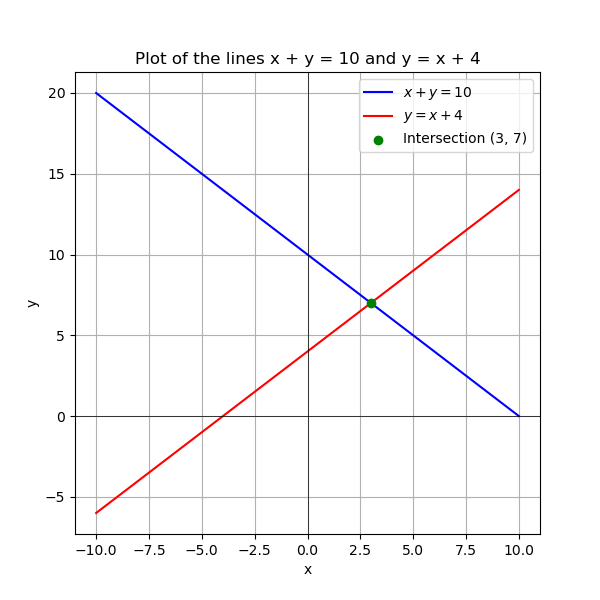
\includegraphics[width=\columnwidth]{figs/Figure_1.png}
	\label{stemplot}
\end{figure}


\end{document}
